
\begin{appendices}
% bei jeder section neue seite beginnen
\newpage
\renewcommand\section{\stdsection}

\addappheadtotoc
\appendixpage


    \section{TXLWizard: Advanced Example}
        \label{sec:AppendixTXLWizardExampleAdvanced}
        The following code demonstrates the usage of ``TXLWizard'' in a more advanved way, including labelling of array objects, nested referencing, etc.
        The generated mask is show in Figure \ref{fig:AppendixTXLWizardExampleAdvanced}.

        \lstinputlisting[language=Python]{Content/Example_GenerateMask.py}


        \begin{figure}[!htbp]
            \centering
             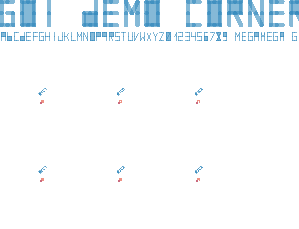
\includegraphics[width=\textwidth]{Content/Masks/EM160509_GOI_Demo_CornerCube.pdf}
            \caption{Advanced Example: Part of the Generated Mask}
            \label{fig:AppendixTXLWizardExampleAdvanced}
        \end{figure}




\end{appendices}